\subsection{Second-Order Optimization (Newton's Method)}

\begin{frame}{Recap: The Limits of First-Order Methods}
    \frametitle{The Problem with a Single Learning Rate}
    \begin{itemize}
        \item Vanilla Gradient Descent uses a single learning rate for all parameters.
        \item On ill-conditioned error surfaces (long, narrow valleys), this is inefficient.
        \item The learning rate is either too large for steep directions (causing oscillation) or too small for shallow directions (causing slow progress).
        \item \textbf{Question:} Can we do better by using information about the surface's curvature?
    \end{itemize}
\end{frame}

\begin{frame}{Second-Order Optimization: The Idea}
    \frametitle{Using Curvature for Faster Convergence}
    Instead of a linear approximation, second-order methods use a local \textbf{quadratic approximation} of the loss function.
    \begin{itemize}
        \item This is based on the second-order Taylor expansion for loss function E($w$) around the current point $w^{(k)}$:
        \begin{equation*}
        \begin{split}
            E(w) \approx E(w^{(k)}) &+ \nabla_{w}E(w^{(k)})^{T}(w-w^{(k)}) \\
            &+ \frac{1}{2}(w-w^{(k)})^{T}H_{E}(w^{(k)})(w-w^{(k)})
        \end{split}
        \end{equation*}
        \item \textbf{Newton's Method} jumps directly to the minimum of this quadratic approximation in a single step.
    \end{itemize}
    \begin{figure}
        % Placeholder for the Newton's method visualization from Optimization II.pdf, p. 4
        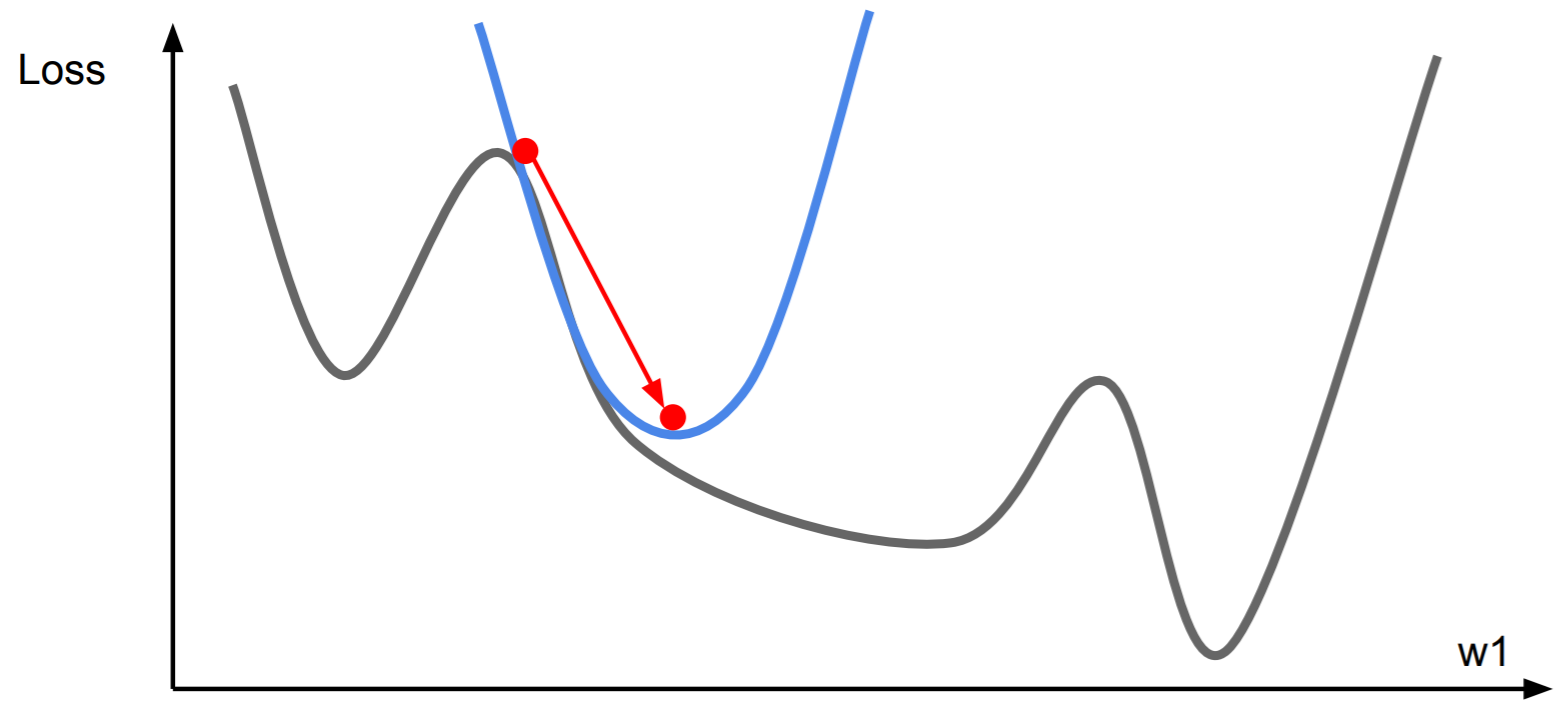
\includegraphics[width=0.5\textwidth]{images/secondmethods.png}
        \caption{Newton's method forms a local quadratic approximation (blue) and jumps to its minimum.}
    \end{figure}
\end{frame}

\begin{frame}{Second-Order Optimization: The Idea}
    \frametitle{Intuition Behind Newton's Method}
    \begin{figure}
        \centering
        \begin{minipage}{.5\textwidth}
            \centering
            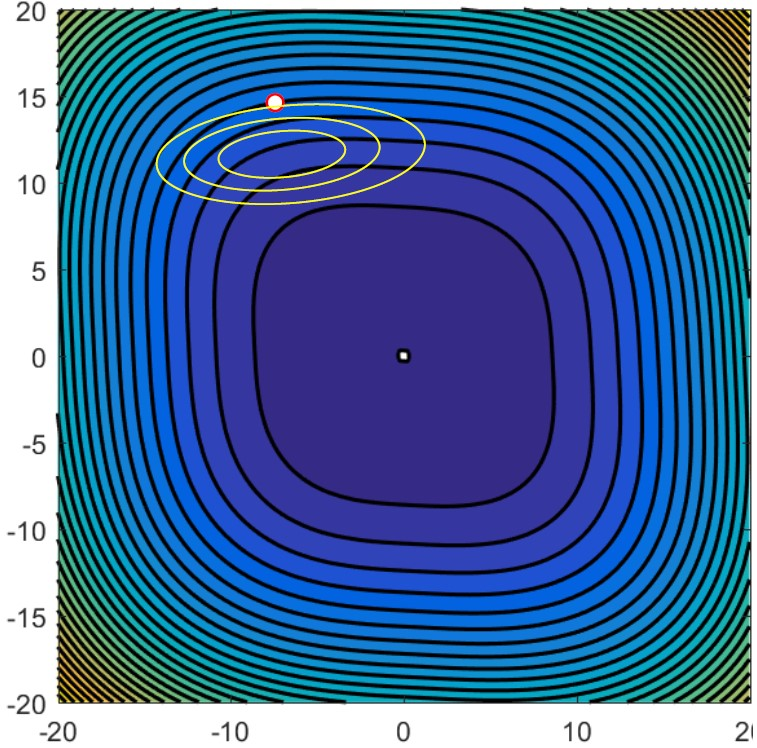
\includegraphics[width=\textwidth]{images/intuition_newton1.jpeg}
        \end{minipage}%
            \begin{minipage}{.5\textwidth}
            \centering
            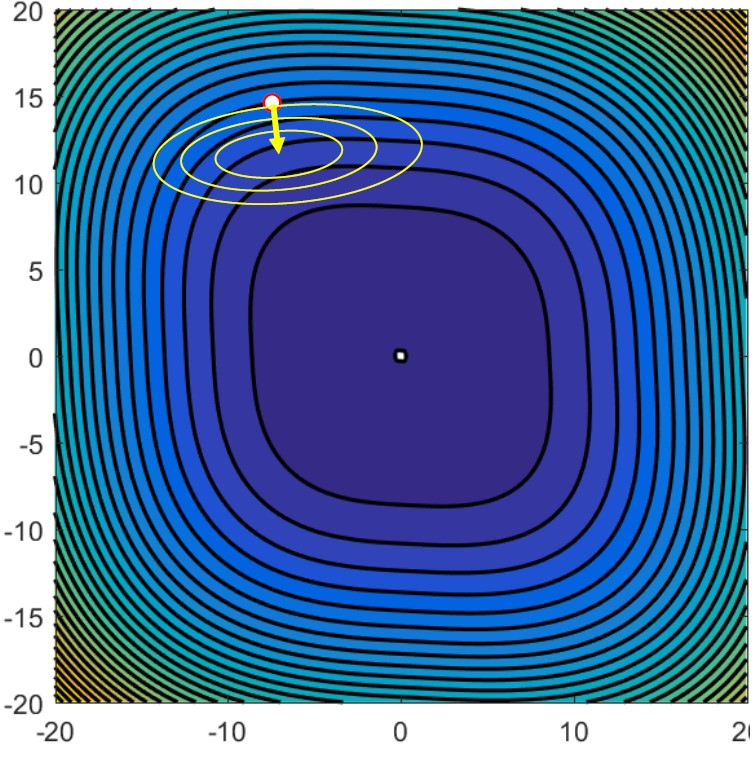
\includegraphics[width=\textwidth]{images/intuition_newton2.jpeg}
        \end{minipage}
    \caption{Fit a quadratic at each point and find the minimum of that quadratic}
    \end{figure}
\end{frame}

\begin{frame}{Newton's Method: The Update Rule}
    \frametitle{Incorporating the Hessian}
    The update rule incorporates the \textbf{Hessian matrix ($H$)}, the matrix of second derivatives, which describes the local curvature.
    \begin{itemize}
        \item The update rule is:
            $$ w^{(k+1)} = w^{(k)} - H_{E}(w^{(k)})^{-1} \nabla_{w}E(w^{(k)}) $$
        \item By multiplying the gradient by the \textbf{inverse Hessian}, the update is rescaled. This effectively transforms the elliptical contours of an ill-conditioned problem into circular ones, allowing for a direct path to the minimum.
        \item For a quadratic function, the optimal $\eta$ is 1 (which is exactly Newton's method). Therefore, this method has no learning rate/hyperparameter to tune; the optimal step size is effectively 1.
    \end{itemize}
\end{frame}



\begin{frame}{Visualizing Second-Order Optimization}
    \frametitle{The Effect of Preconditioning}
    
    \begin{figure}
        \centering
        % This tikzpicture environment manually places all elements
        \begin{tikzpicture}
            % Define coordinates for the center of each image
            \coordinate (pos1) at (-3.5, 5.5);
            \coordinate (pos2) at (3.5, 5.5);
            \coordinate (pos3) at (-3.5, 2);
            \coordinate (pos4) at (3.5, 2);
            
            % Place the images as nodes at the defined positions
            \node at (pos1) {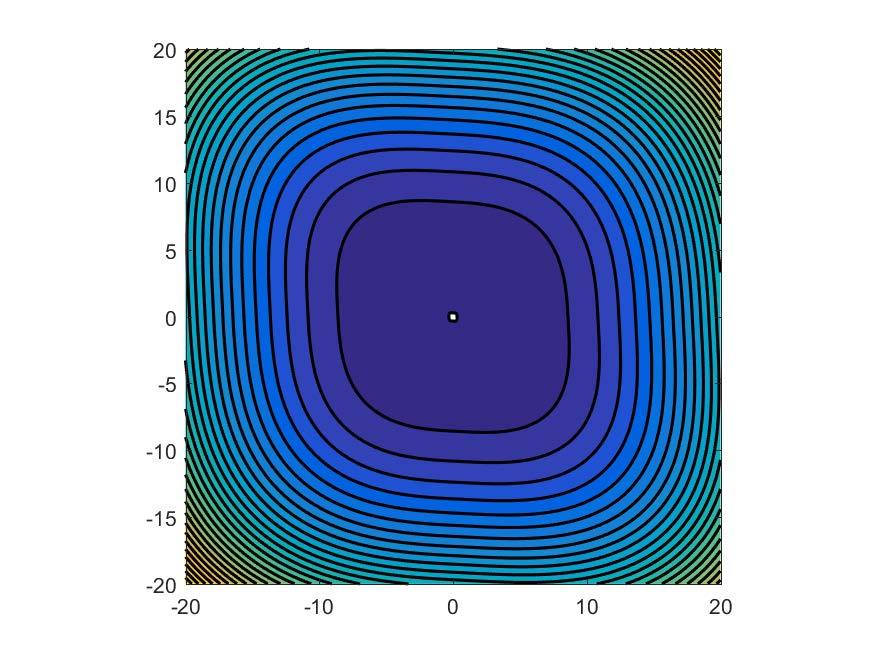
\includegraphics[width=0.4\textwidth]{images/contour_before_seocnd.jpeg}};
            \node at (pos2) {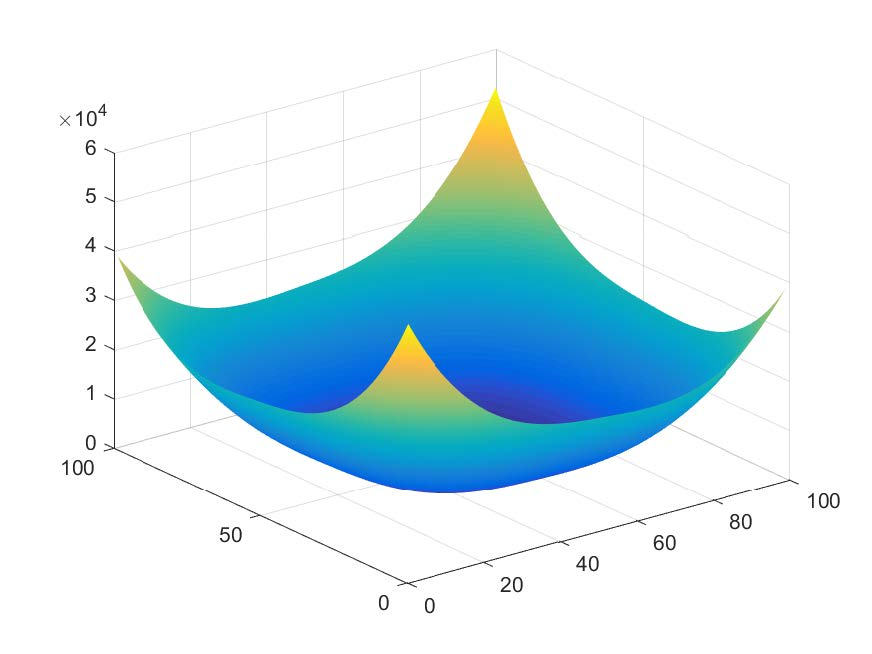
\includegraphics[width=0.4\textwidth]{images/loss_before_second.jpeg}};
            \node at (pos3) {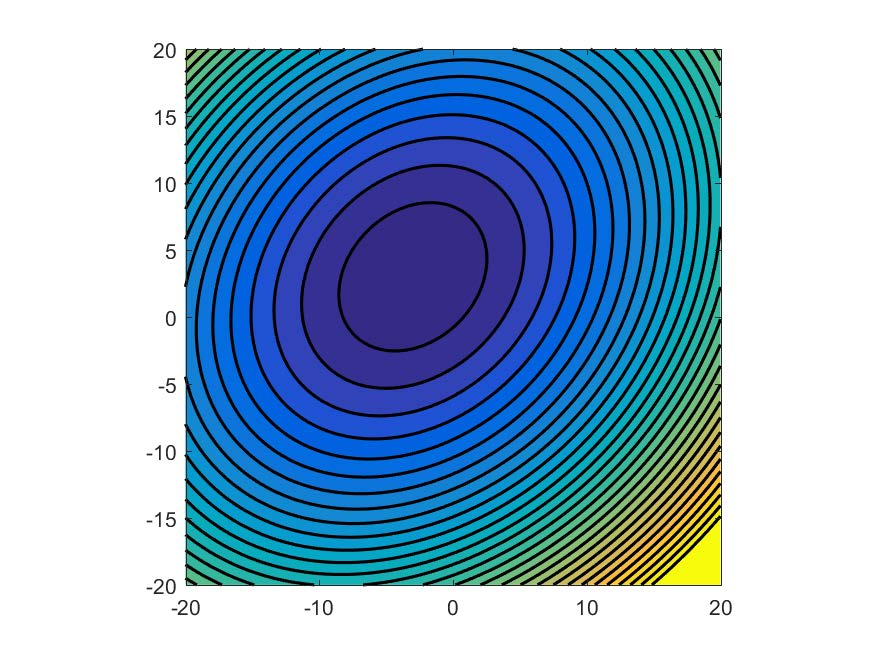
\includegraphics[width=0.4\textwidth]{images/contour_after_second.jpeg}};
            \node at (pos4) {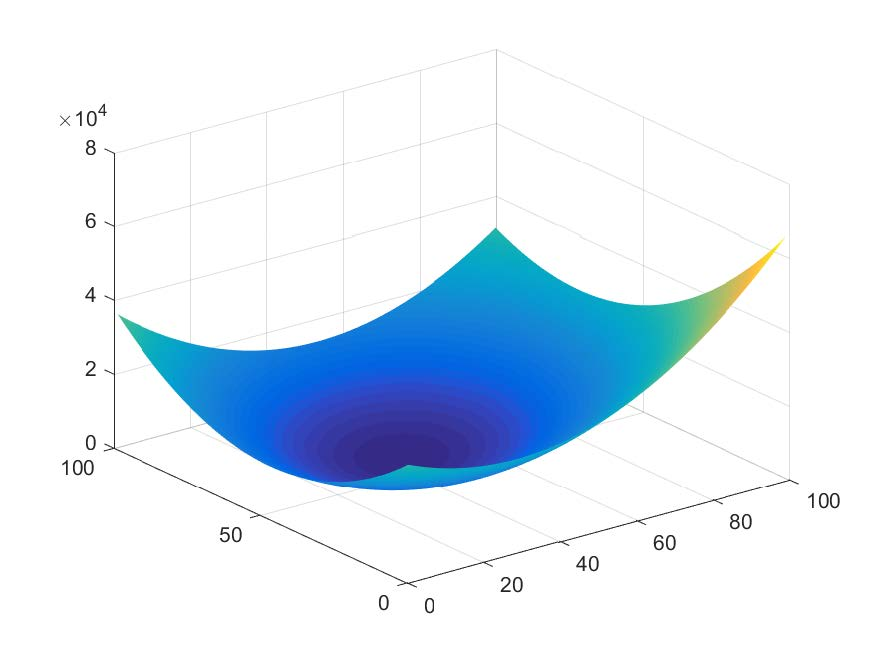
\includegraphics[width=0.4\textwidth]{images/loss_after_second.jpeg}};
            
            % Define the start and end points for the arrow, centered horizontally
            \coordinate (arrow_start) at (0, 5);
            \coordinate (arrow_end) at (0, 3);
            
            % Draw the arrow using the standard -> tip
            \draw[->, ultra thick, blue!60!white, line width=2pt] 
                (arrow_start) -- (arrow_end);
        \end{tikzpicture}
        \caption{Visualizing the error surface before (top) and after (bottom) applying second-order information.}
    \end{figure}
    
\end{frame}





\begin{frame}{The Drawbacks of Newton's Method}
    \frametitle{Why It's Impractical for Deep Learning}
    Despite its rapid convergence, Newton's method is not used for large-scale deep learning.
    \begin{itemize}
        \item \textbf{Prohibitive Computational Cost}:
        \begin{itemize}
            \item For a network with $n$ parameters, the Hessian matrix has $n^2$ elements.
            \item Calculating the Hessian takes $O(n^2)$ time.
            \item Inverting it takes $O(n^3)$ time. For millions of parameters, this is infeasible.
        \end{itemize}
        \item \textbf{Stability Issues on Non-Convex Surfaces}:
        \begin{itemize}
            \item For non-convex functions, the Hessian may not be positive definite. This can cause the update to move towards a saddle point or maximum instead of a minimum.
        \end{itemize}
    \end{itemize}
\end{frame}

\begin{frame}{Quasi-Newton Methods: A Practical Compromise}
    \frametitle{Approximating the Inverse Hessian}
    \begin{itemize}
        \item \textbf{Quasi-Newton methods}, like BFGS, avoid the full computation of the inverse Hessian.
        \item They iteratively build up an approximation of the inverse Hessian using only first-order gradient information.
        \item \textbf{L-BFGS (Limited-memory BFGS)} is a popular variant that uses only the last few gradient updates, making it more memory-efficient.
        \item However, L-BFGS works best in a full-batch, deterministic setting and does not transfer well to the noisy, mini-batch updates common in deep learning.
    \end{itemize}
    \begin{alertblock}{Next Steps}
        Since second-order methods are too costly, we look for more sophisticated first-order methods that can tackle the conditioning problem without computing the Hessian.
    \end{alertblock}
\end{frame}
